\section{Mikrokontroliers un vadības sistēma caur tīklu}
Kā mikrokontrolieris tika izvēlēts W5500-EVB-Pico \cite{pico}, balstoties uz darba vadītāja ieteikumu, kam ir TCP/IP tīkla steka atbalsts, ar kuru ir gatavi TCP servera piemēri, kas saņem un nosūta komandas tīklā, kā arī mikrokontrolierim ir divi kodoli.
\begin{figure}[H]
	\centering
    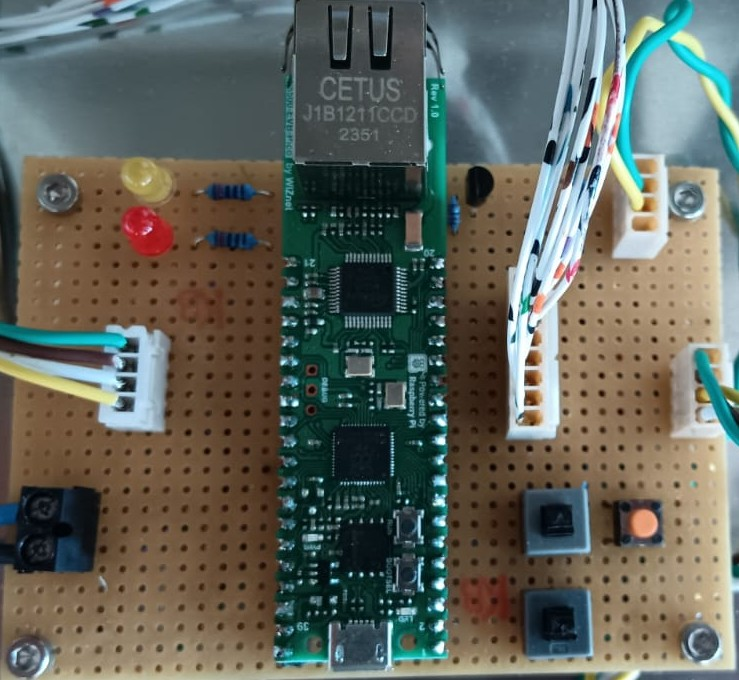
\includegraphics[width=0.6\textwidth]{pictures/mcu_board.jpg}\hspace{1cm}
    \caption{Mikrokontroliera iespiedplate}
\end{figure}
RP4020 mikrokontrolieris tiek plaši pielietots iegultajās sistēmās, jo viena mikroshēma satur CPU, atmiņu, RAM, watchdogs u.c. perifērijas. Tika izvēlēts Arduino IDE šim mikrokontrolierim, izmantojot C un C++ programmēšanas valodas. Arduino vide tika izvēlēta dēļ gatavo bibliotēku pieejamības WS5500 tīkla modulim \cite{ws5500}, un VSRC izstrāde ir balstīta uz šīm bibliotēkām.
\begin{figure}[H]
	\centering
    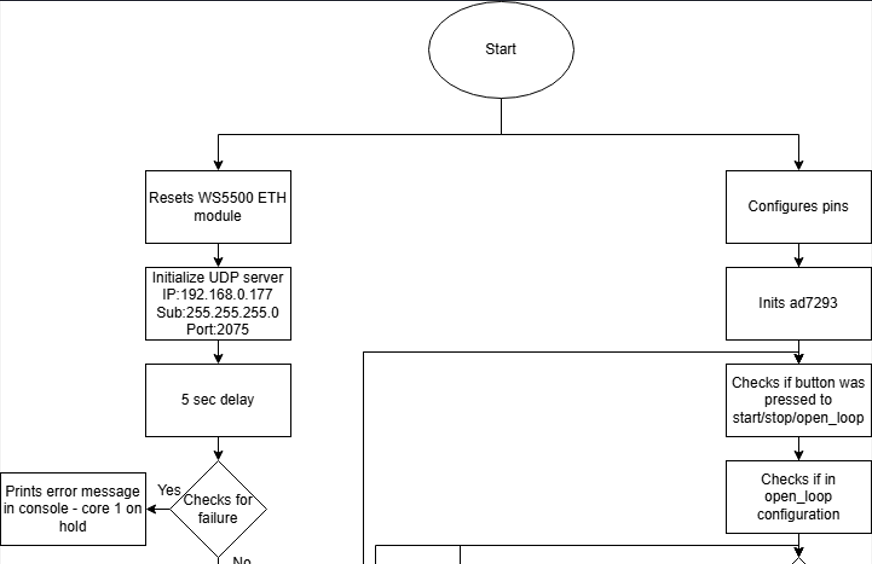
\includegraphics[width=0.8\textwidth]{pictures/prog_code_1.png}\hspace{1cm}
    \caption{Daļa no programmas koda bloka diagramma}
\end{figure}
Divkodolu mikrokontrolierim tiek izmantots viens kodols servera uzturēšanai un datu pārraidei, bet otrā tiek kontrolēti mikrokontroliera izvadi, monitorēšanas integrālā shēma, temperatūras mērīšana un sistēmas statusa noteikšana. Programmas kods sākas ar to, ka pirmajā kodolā tiek restartēts un konfigurēts WS5500 modulis, tad tiek konfigurēts izvadīts kļūdas paziņojums, tas tiek darīts 3 reizes un pēc trešās reizes, ja nesanāk, tad kodols tiek apstādināts. Otrā kodolā nokonfigurē izvadus un darba punkta un monitorēšanas integrālo shēmu. Tad tiek pārbaudīts, vai ir nospiesta viena no trim pogām. Spiedpogas paredzētas manuālai testēšanai, kur pirmā spiedpoga atbild par sistēmas ieslēgšanu un darba punkta nodrošināšanu, otrā spiedpoga nodrošina sistēmas izslēgšanu un darba punkta atiestatīšanu, bet trešā, lai deaktivizētu slēgto ciklu, lai varētu pārraidīt RF signālu ar mainīgu jaudu. Tiek pārbaudīts, vai ir atvērtā cikla konfigurācijā, ja jā, tad tiek aktivizēta gaismas diode, kas atrodas uz mikrokontroliera plates.
\begin{figure}[H]
	\centering
    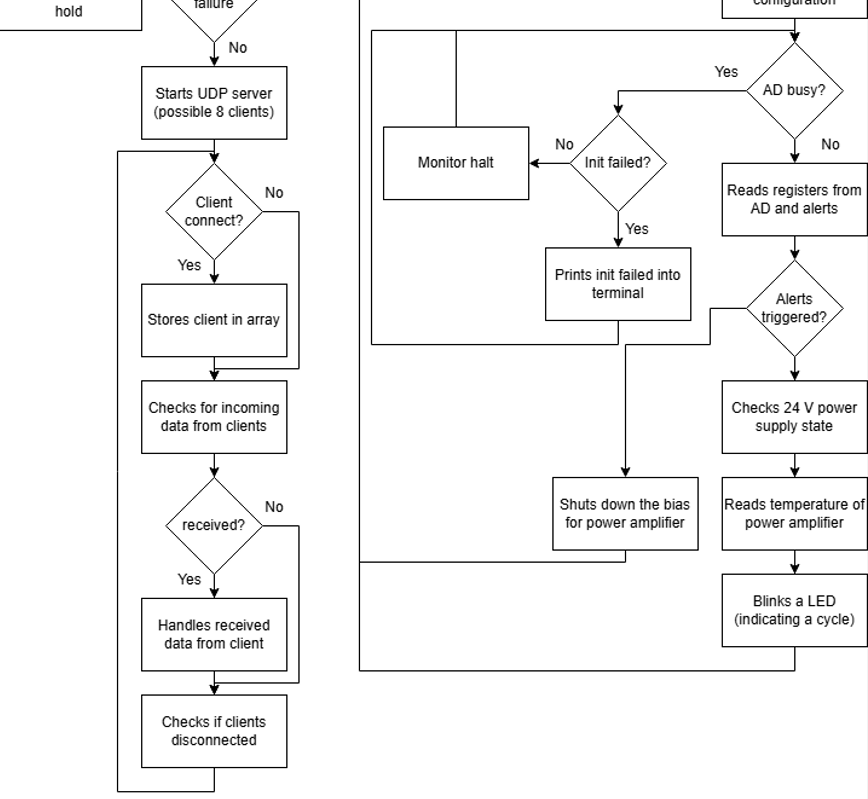
\includegraphics[width=0.8\textwidth]{pictures/prog_code_2.png}\hspace{1cm}
    \caption{Daļa no programmas koda bloka diagramma}
\end{figure}
Pirmajā kodolā tiek uzsākts serveris, pie kura var pieslēgties līdz astoņiem klientiem. Pirmajā kodolā tiek pārbaudīts, vai ir jauns klienta pieslēgšanās pieprasījums, ja ir, tad klienta TCP objektu saglabā masīvā, kas glabā informāciju par klienta IP adresi un portu, kā arī savienojuma stāvokli, bet, ja nav, tad pārbauda, vai ir saņemti komandas no klientiem, ja tādi ir, ja kādi dati ir saņemti, tad to apstrādā un veic attiecīgu darbību, bet, ja nav, tad pārbauda, vai kāds klients ir atslēdzies no servera, lai varētu atbrīvot masīvu un vietu citam klientam. Otrā kodolā tiek pārbaudīts, vai monitorēšanas integrālā shēma ir aizņemta, tas datu lapā netiek uzsvērts, bet pārbaude netraucē, ja ir, tad pārbauda, vai tā tiek izmantota citā procesā vai ir inicializācijas problēmas, tad pārbauda tās statusu atkal. Ja AD7293 ir gatavs komunikācijai, tad tiek nolasīti reģistri un karodziņi, ja kāds no karodziņiem tiek aktivizēts, tad darba punktu atiestata un atslēdz sistēmu, bet, ja nav, tad tiek pārbaudīts 24 V elektrobarošanas statuss, nolasīta temperatūra un ieslēdz un ar aizskavi izslēdz gaismas diodi, kas atspoguļo viena cikla beigas.\\
Mikrokontrolieris saglabā sistēmas esošo stāvokli mainīgajā, nolasa datus no sensoriem un monitorēšanas integrālās shēmas datus, kuri tiek strukturizēti simbolu virknē un nosūtīti caur TCP protokolu klientam pēc pieprasījuma. Zemāk apkopota telemetrijas virkne.
\begin{table}[H]
\centering
\captionsetup{singlelinecheck=off, justification=raggedleft}
\caption{Telemetrijas virknes struktūra un atšifrējums}
\renewcommand{\arraystretch}{1.2}
\begin{tabular}{|c|c|l|l|}
\hline
\multirow{24}{*}{\centering 96 baiti} & \textbf{Datu tips} & \textbf{Mainīgā nosaukums} & \textbf{Definīcija} \\
\hline
\cline{2-4}
& I    & pa\_on\_state          & HPA stāvoklis (0=off, 1=on) \\
\cline{2-4}
& I    & psu\_pg\_state         & Barošanas avota status (0=off, 1=on) \\
\cline{2-4}
& I    & open\_loop\_mode       & Kontroles režīms (0=closed, 1=open) \\
\cline{2-4}
& F    & rs0\_volts            & Noteces spriegums HPA \\
\cline{2-4}
& UI   & rs\_alert\_high       & Maksimālā noteces slieksņa brīdinājums\\
\cline{2-4}
& UI   & rs\_alert\_low        & Minimālā noteces slieksņa brīdinājums\\
\cline{2-4}
& UI   & alert0\_state         & Sistēmas brīdinājumu status \\
\cline{2-4}
& F    & isense0\_amps         & Strāvas mērījums 0 kanālam\\
\cline{2-4}
& F    & isense1\_amps         & Strāvas mērījums 1 kanālam\\
\cline{2-4}
& F    & Ug0\_volts            & Aizvara sprieguma 0 mērījums \\
\cline{2-4}
& F    & Ug0\_volts\_lim       & Aizvara sprieguma 0 limits \\
\cline{2-4}
& F    & Ug1\_volts            & Aizvara sprieguma 1 mērījums \\
\cline{2-4}
& F    & Ug1\_volts\_lim       & Aizvara sprieguma 1 limits \\
\cline{2-4}
& F    & temp\_degC            & Temperatūra korpusā \\
\cline{2-4}
& F    & temp1\_degC           & Temperatūra uz HPA 1 \\
\cline{2-4}
& F    & temp2\_degC           & Temperatūra uz HPA 2 \\
\cline{2-4}
& F    & temp\_degC\_Fpwr      & Izstarotā jaudas mērītāja temperatūra \\
\cline{2-4}
& F    & temp\_degC\_Rpwr      & Atstarotās jaudas mērītāja temperatūra\\
\cline{2-4}
& F    & temp\_degC\_AD7293      & Monitorēšanas IC temperatūra\\
\cline{2-4}
& F    & reflected\_power\_log      & Atstarotā jauda dBm \\
\cline{2-4}
& F    & reflected\_power\      & Atstarotā jauda W\\
\cline{2-4}
& F    & forward\_power\_log        & Izstarotā jaudas dBm \\
\cline{2-4}
& F    & forward\_power\        & Izstarotā jaudas W \\
\cline{2-4}
& F    & $S_{11}$\_param\        & Izstarotā jaudas W \\
\hline
\end{tabular}
\end{table}
 Struktūra sastāv no 96 baitiem. Pirmie 4 baiti satur esošo jaudas pastiprinātāja stāvokli (izslēgts, ieslēgts), otrie 4 baiti satur 24 V elektrobarošanas statusu (ieslēgts, izslēgts), trešie 4 baiti satur informāciju par to, vai ir cikla konfigurācijā, ceturtie 4 baiti, kas atgriež sprieguma kritumu uz šunta rezistora, tad nākošie 4 baiti atgriež karodziņu vecāko un jaunāko baitu, tad nākošie četri ir karodziņi. Isens0 atgriež strāvas vērtību caur pirmo šunta rezistoru, kur Isense1 atgriež strāvas vērtību caur otro šunta rezistoru. Tālāk iet UG0 volti, kas nosaka, kāds ir aizvara vadības sprieguma līmenis pirmajam pastiprinātājam, tad ir ierobežojums, kas nosaka iestatītās robežvērtības, tad nākošie 8 baiti nozīme ir ekvivalenta tikai otram pastiprinātājam. Nākošie 4 baiti ir temperatūras mērījums korpusā, tad 8 baiti ir temperatūras mērījumi divos punktos uz jaudas pastiprinātāja, tad nākošie 8 baiti ir jaudas mērītāju IC temperatūra izstarotajai un atstarotajai jaudai un 4 baiti monitorēšanas IC temperatūra. Nākošie 16 baiti ir izstarotās un atstarotās jaudas logaritmiskā un matemātiskā reprezentācijā. Pēdējais ir S11 parametrs.\\
 Klients var nosūtīt vairākas komandas mikrokontrolierim, lai iestatītu režīmu, mainītu konfigurāciju un pieprasītu datus.
 \begin{table}[H]
\centering
\captionsetup{singlelinecheck=off, justification=raggedleft}
\caption{Iespējamās komandas un to atšifrējums}
\renewcommand{\arraystretch}{1.2}
\begin{tabular}{|c|c|l|l|}
\hline
\multirow{6}{*}{\centering 15 baiti} & \textbf{Datu tips} & \textbf{Mainīgā nosaukums} & \textbf{Definīcija} \\
\hline
\cline{2-4}
& S    & mon          & Pieprasa telemetrijas virkni \\
\cline{2-4}
& S    & pon          & Aktivizē/deaktivizē sistēmu \\
\cline{2-4}
& S    & olm          & Maina noslēgtās cilpas konfigurāciju \\
\cline{2-4}
& S    & setcurr          & Iestata noteces strāvu kanāliem \\
\cline{2-4}
& S    & setramp          & Iestata darba punkta iestatīšanas periodu \\
\hline
\end{tabular}
\end{table}
Maksimālā simbola virkne, ko var apstrādāt mikrokontrolieris, ir 15 baiti. Mon komanda ir vienīgā, kura nepieņem papildus argumentus, mikrokontrolieris saņemot šo komandu, atbild nekavējoties ar telemetrijas virkni klientam. Pon komanda pieņem vienu argumentu 0 vai 1, ja tiek saņemts 1, tad tiek uzsākta sistēmas darbība (elektrobarošanas ieslēgšana, darba punkta nodrošināšana u.c.), bet, ja saņem 0, tad sistēmas darbība tiek pārtraukta (darba punkta atiestatīšana, elektrobarošanas izslēgšana u.c.). Olm komanda pieņem vienu argumentu 0 vai 1, ja saņemts ir 1, tad slēgtais cikls tiek izslēgts, ja saņem 0, tad to aktivizē. Ja tiek padoti nepareizi ieejas argumenti, tad sistēma atbild ar iespējamajiem variantiem lietotājam. Setcurr komanda pieņem peldošā komata mainīgo, kas iestata darba punkta strāvu visiem kanāliem. Setramp pieņem float argumentu, ar kuru var izmainīt darba punkta noturēšanas strāvu no 250~\textmu s līdz 31.75~ms
\begin{figure}[H]
	\centering
    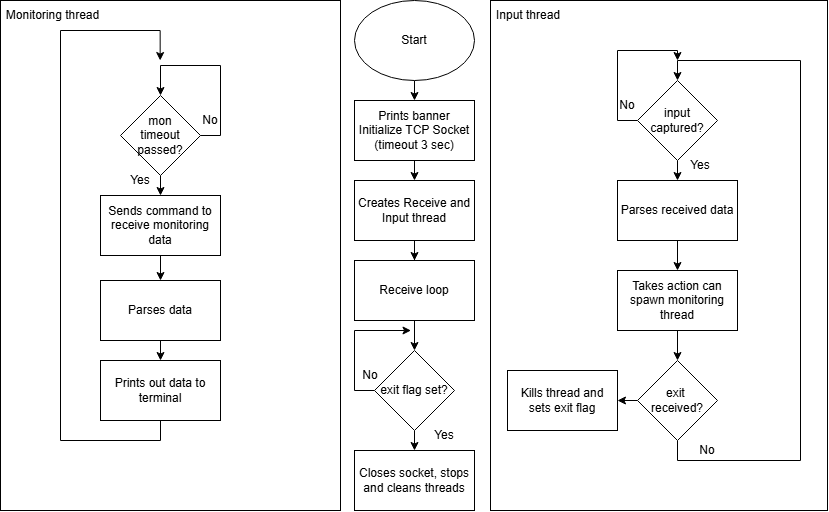
\includegraphics[width=0.8\textwidth]{pictures/script_program.drawio.png}\hspace{1cm}
    \caption{Python skripta bloka diagramma}
\end{figure}
Tika izveidots Python skripts uz Windows 11 OS, kas uzsāk X-joslas sistēmas darbību. Skriptu startējot, tiek terminālī izvadīts logo, atšifrējums, sistēmas nosaukums un palīginstrukcija ar visām iespējamām darbībām. Tad tiek izveidots TCP klients, kurš mēģina pieslēgties pie TCP servera ar 3 sekunžu intervālu; ja neizdodas, skripts beidz savu darbu. Kad ir izveidots savienojums ar serveri, tad skripts izveido ievades pavedienu un ieiet uztveršanas ciklā. Uztveršanas cikls gaida ienākošo simbolu virkni un saņemšanas brīdī to izvada; ja nekas netiek saņemts, tad tiek izvadīts paziņojums, ka serveris ir pārtraucis kontaktēties, un beidzas skripta darbība. Ievades pavedienā tiek termināli izvadīts teksts ar aicinājumu uzsākt sistēmas darbību ar "start", kas uzsāk X-joslas sistēmas darbību, aktivizējot sistēmu un iestatot darba punktu ar noklusējuma vērtībām. Kad tiek saņemta simbolu virkne, tā tiek pārbaudīta, vai virkne atbilst kādai no iespējamajām funkcijām; ja nē, tas tiek automātiski nosūtīts mikrokontrolierim. Ja komanda atbilst kādai no skripta funkcionalitātēm, tad tā tiek parsēta un attiecīgi izvadīta informācija vai pārtraukta tās darbība. Kad tiek nosūtīta start komanda, skripts izveido monitorēšanas pavedienu, kur ik pēc iestatītā intervāla tiek veikta telemetrijas virknes nolase no mikrokontroliera, tad ienākošā telemetrija tiek parsēta un izvadīta lietotājam ērtākā virtenē. Ja tiek saņemta "exit" komanda vai ctrl+c kombinācija, tad automātiski sistēma pārtrauc savu darbību un pārbauda, vai kāds no pavedieniem ir aktīvs; ja ir, tad to pārtrauc, kā arī tiek pārbaudīts sistēmas stāvoklis; ja tas ir ieslēgts, tad to izslēdz pirms skripts aizveras.